\documentclass[a4paper,pagesize 10pt]{scrartcl}

\usepackage{graphicx}
\usepackage{scalefnt}
\usepackage{textfit}

\begin{document}


\begin{center}{\Huge\textbf{Project Proposal}}\end{center}
\begin{center}{\Large\textbf{Face reconstruction}}\end{center}

\section{Abstract}
The target of our project is to implement a functionality that fits RGB-D data to a human face model.\\
The first step is to gather the RGB-D data using a Kinect camera. The built-in RGB cameras and depth sensors are optimally suited for this task.
Following we backproject and preprocess the raw RGB-D data to produce a point cloud of vertices with assigned color and normal values. 
Based on this point cloud we will use parameter estimation to find the optimal rotation and translation parameters to estimate the head pose and the warp parameters. 
To find a good fit for the face model we will search for characteristic features in the point cloud and use these as additional parameters to warp the face model.
Finally we will create a realistic 3D face model of the scanned person.\\
We will base our research on the works described in \cite{Bondi2015, Shin2017, Turban2015,Zhang2016,Zollhofer2014}.

\begin{figure}[h]
	\centering
	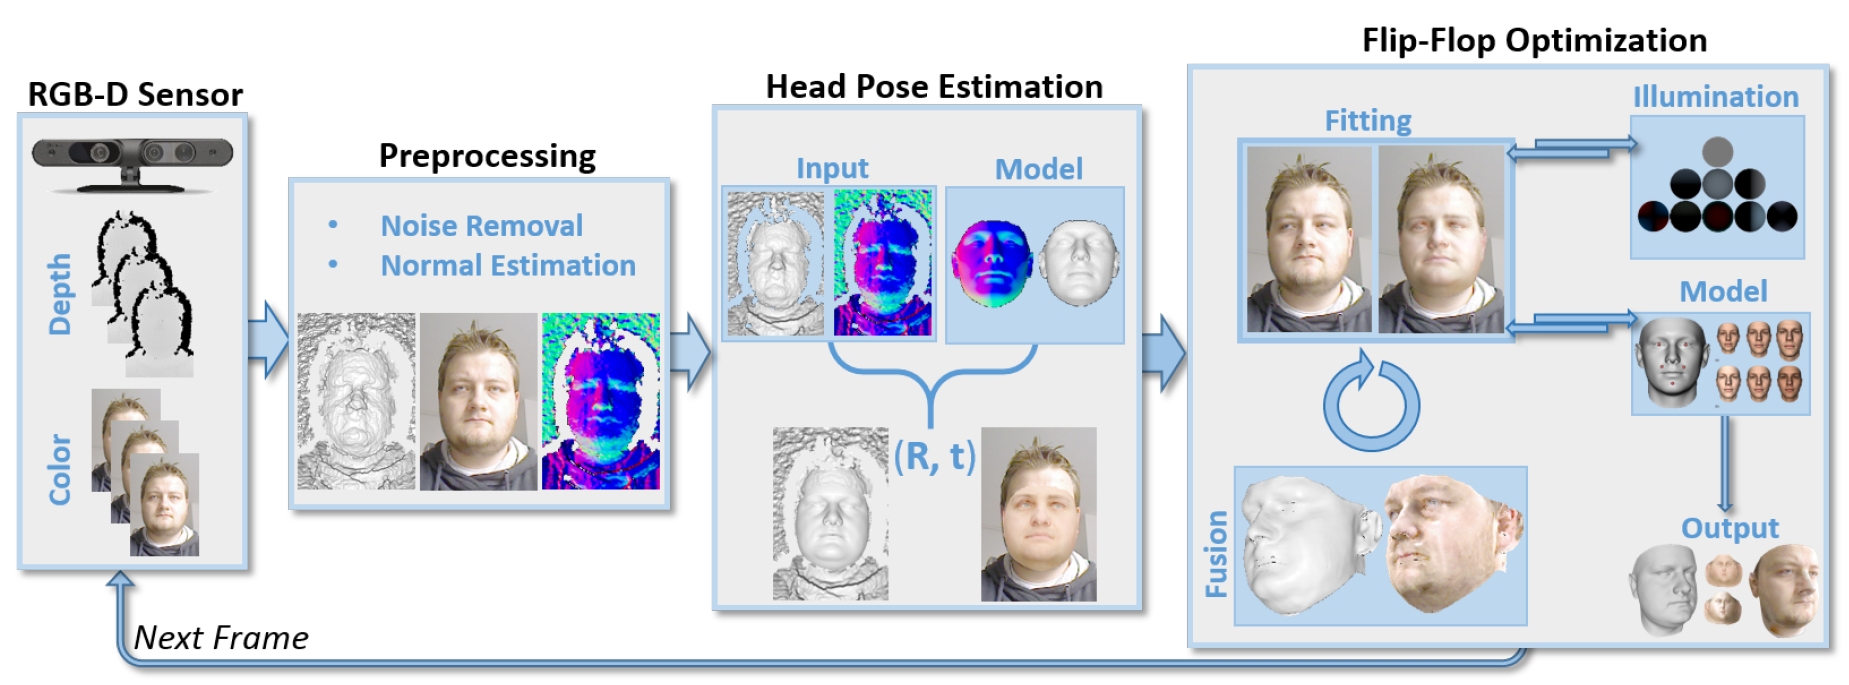
\includegraphics[width=\linewidth]{Images/pipeline.png}
	\caption{An exemplary processing pipeline. We start by gathering the RGB-D data from the Kinect. Following we preprocess the raw RGB-D data and estimate the head pose. Finally we will fit the face mode to the captured RGB-D data.
	We omit the last step of Flip-Flop optimization and only warp the face model according to the detected face features.}
	\label{fig:overview}
\end{figure}

\section{Requirements}
\begin{itemize}	
	\item Kinect sensor
\end{itemize}

\section{Team}
Marcel Bruckner, Kevin Bein, Jonas Schulz, Chandramohan Sudar

\section{Weekly milestones}
\begin{enumerate}
	\item Gathering of the RGB-D data from the Kinect sensor
	\item Backprojection of depth and RGB data to world space and generation of the point cloud
	\item Filtering and enhancing of the produced point cloud and background segmentation
	\item Find characteristic points in the point cloud to fit the face model
	\item Fitting of the face model
	\item Generation of a high resolution 3D face reconstruction
\end{enumerate}

% references
{\small
	\bibliographystyle{plain}
	\bibliography{Literature/3D-Scanning}
}

\end{document}


